\section{Løsninger til linære programmeringsproblemer}

Den mulige mængde er mængden af løsningsvektorer, $\vec{x}$, som opfylder alle problemets betingelser. Hvis en optimal løsning eksisterer vil denne derved være indeholdt i den mulige mængde.

\begin{defn}[Mulige løsninger og den mulige mængde]
En \textbf{mulig løsning} er en løsningsvektor $\vec{x}$, som opfylder alle problemets betingelser.\\
\textbf{Den mulige mængde} $\mathcal{F}$ er mængden af alle de mulige løsninger. Den vil derfor, for et standard maksimumsproblem være defineres som
\begin{align*}
\mathcal{F}=\{\vec{x} \in \mathds{R}^n|A\vec{x} \leq \vec{b}, \vec{x} \geq \vec{0}\}
\end{align*}
%En vektor $\vec{x}^*$ kaldes en \textbf{optimal løsning}, hvis 
%\begin{align}
%	f(\vec{x}^*)=\max\limits_{\vec{x} \in \mathcal{F}}f(\vec{x}).
%\end{align}
Et problem kaldes \textbf{inkonsistent} (usikker på oversættelse) hvis den mulige mængde er den tomme mængde, ellers er problemet \textbf{konsistent}. %Et problem kaldes \textbf{ubegrænset}, hvis objektfunktionen kan tage arbitrært store funktionsværdier for maksimeringsproblemer, og arbitrært små funktionsværdier for minimeringsproblemer. Ellers kaldes problemet \textbf{begrænset}.
\end{defn}
%Linje efter align og \\ skal enten skrives i bindende tekst eller gøres mere præcis

%Den optimale løsning kan findes på forskellige måder heriblandt med simplex-metoden, som beskrives i senere kapitler. En anden måde er ved geometrisk visualisering af den mulige mængde. Denne metode er mulig for problemer med op til 3 variable, da løsningsmængden derved visualiseres som et plot i det tilsvarende antal dimensioner. 

\begin{eks}[Den mulige mængde]
Ved at indtegne betingelserne i et koordinatsystem, er det muligt at visualisere den mulige mængde som fællesmængden af de mængder, der dannes ud fra betingelserne. På Figur \ref{fig:maksprob2} er den mulige mængde for problemet i Eksempel \ref{eks:maksprob2} indtegnet. Der er desuden tegnet en pil for hver betingelse, som viser for hvilken side af linjen, at koordinaterne opfylder betingelsen. Den mulige mængde er farvet grå.

\begin{center}
	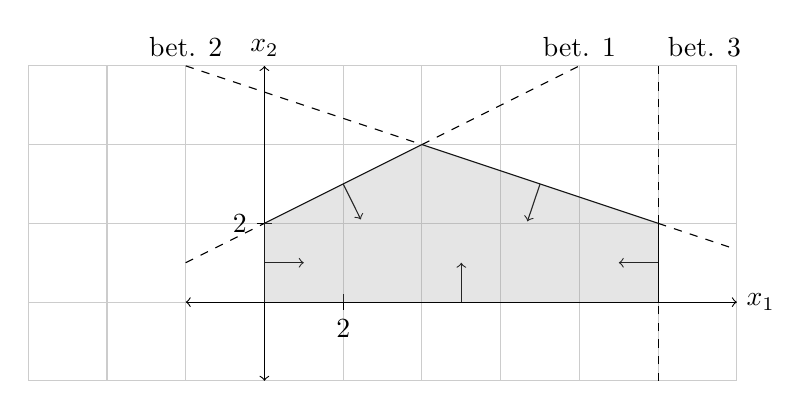
\begin{tikzpicture}
  %laver Grid. godt til når koordinater skal redigeres
  	\draw[thin,gray!40] (-3,-1) grid (6,3); 
  %x-aksen
  	\draw[<->] (-1,0)--(6,0) node[right]{$x_1$};
  	\draw[->] (2.5,0) -- (2.5,0.5);
  %y-aksen
  	\draw[<->] (0,-1)--(0,3) node[above]{$x_2$};
  	\draw[->] (0,0.5) -- (0.5,0.5);
  	
  %akse-markeringer
  	%\node[left] (xakse) at (0,1) {2};
  	\draw[] (-0.1,1) -- (0.1,1) node[pos=0,left] {2};
  	\draw[] (1,-0.1) -- (1,0.1) node[pos=0,below] {2};
  	
  %ligning 1
	\draw[domain=-1:0,variable=\x,dashed] 	plot({\x},{0.5*\x+1});
	\draw[domain=0:2,variable=\x] 			plot({\x},{0.5*\x+1});
	\draw[domain=2:4,variable=\x,dashed] 	plot({\x},{0.5*\x+1}) node[above] {bet. 1};
  	\draw[->] (1,1.5) -- (1.224,1.05);
	
  %ligning 2
  	\draw[domain=-1:2,variable=\x,dashed] 	plot({\x},{-(1/3)*\x+8/3}) node[above] at (-1,3) {bet. 2} ;
	\draw[domain=2:5,variable=\x] 			plot({\x},{-(1/3)*\x+8/3});
	\draw[domain=5:6,variable=\x,dashed] 	plot({\x},{-(1/3)*\x+8/3});
	\draw[->] (3.5,1.5) -- (3.34,1.026);

  %ligning 3
  	\draw[domain=-1:0,variable=\y,dashed] 	plot({5},{\y});
	\draw[domain=0:1,variable=\y] 			plot({5},{\y});
	\draw[domain=1:3,variable=\y,dashed] 	plot({5},{\y}) node[above right] {bet. 3};
	\draw[->] (5,0.5) -- (4.5,0.5);

  %løsningsmængden skraveret
	\fill[gray!80,nearly transparent] (0,0) -- (0,1) -- (2,2) -- (5,1) --(5,0) --  cycle;
\end{tikzpicture}
	\captionof{figure}{Skravering af den mulige mængde for et standard maksimeringsporblem.}
	\label{fig:maksprob2}
\end{center}

\end{eks}